\chapter{PROPOSTA}
\label{chap:proposta}

Este capítulo detalha a proposta para abordar o problema apresentado na seção \ref{chap:introducao}

\section{O protocolo SPolKA}

O protocolo \nome\ estende a arquitetura de roteamento na origem baseada em sistemas de numeração de resíduos (\textit{Residue Number System} -- RNS) \cite{Shoup:2009,dominicini2020} ao incorporar, de forma nativa e sem estados no núcleo, o escalonamento de pacotes orientado a classes de serviço. Enquanto abordagens tradicionais de roteamento na origem baseadas em empilhamento de rótulos exigem que cada salto remova ou atualize o cabeçalho --- incorrendo em sobrecarga crescente proporcional ao diâmetro da rede ---, o \nome\ codifica toda a trajetória e as respectivas políticas de Qualidade de Serviço (QoS) em um único identificador compacto e imutável ao longo do núcleo.

\subsection{ARQUITETURA DO SPOLKA}

O funcionamento da arquitetura divide-se logicamente em três etapas principais: (i) a atribuição de identificadores e o cálculo do rótulo no Plano de Controle; (ii) a classificação e o encapsulamento na borda de ingresso; e (iii) o encaminhamento e o enfileiramento sem estados nos comutadores de núcleo.

Para formalizar o processo de codificação, considere um fluxo de tráfego que deve atravessar um caminho selecionado composto por $N$ nós de núcleo. Na fase de inicialização da topologia, o Controlador atribui a cada comutador de núcleo um identificador único representado por um polinômio $s_i(t)$ sobre o corpo finito de Galois $GF(2)$, formando o conjunto ordenado $S = \{s_1(t), s_2(t), \ldots, s_N(t)\}$ dos \nodeIDs\ ao longo do trajeto. Para garantir a unicidade da solução matemática, os polinômios pertencentes ao conjunto $S$ devem ser necessariamente coprimos entre si.

Simultaneamente, o Controlador define as ações de encaminhamento e priorização que cada nó intermediário deverá executar. Para cada salto $i \in \{1, 2, \ldots, N\}$, estabelece-se um polinômio de saída $o_i(t)$, pertencente ao conjunto $O = \{o_1(t), o_2(t), \ldots, o_N(t)\}$. Diferentemente da abordagem original do PolKA, na qual o resíduo codifica exclusivamente a interface de egresso, no \nome\ o polinômio $o_i(t)$ resulta da concatenação binária entre o identificador da porta física de saída (\portID) e o identificador da fila de serviço (\qID) atribuída ao fluxo naquele nó. Para que a recuperação dessa informação ocorra sem ambiguidades na operação de módulo, cada par de polinômios deve satisfazer estritamente a restrição de grau dada por $\text{grau}(s_i) > \text{grau}(o_i)$.

De posse dos conjuntos $S$ e $O$, o Controlador sintetiza o identificador global da fatia e da rota, denominado \routeID\ e representado pelo polinômio $R(t)$, por meio da aplicação do Teorema Chinês dos Restos (CRT, do inglês \textit{Chinese Remainder Theorem}) polinomial \cite{Shoup:2009, dominicini2020}. O polinômio $R(t)$ é calculado de modo a satisfazer simultaneamente o seguinte sistema de congruências lineares em $GF(2)$:

\begin{equation}
R(t) \equiv o_i(t) \pmod{s_i(t)}, \quad \forall i \in \{1, 2, \ldots, N\}
\end{equation}

Uma vez computado o \routeID, o Controlador traduz a política de engenharia de tráfego instalando regras de correspondência (\textit{match-action}) exclusivamente nos comutadores de borda da rede. No nó de ingresso, o tráfego entrante é classificado com base em metadados de serviço --- tais como o identificador de fatia S-NSSAI em arquiteturas 5G/6G ou marcações DiffServ --- e associado ao respectivo \routeID, que é então inserido no cabeçalho do pacote. Graças às propriedades aritméticas dos polinômios sobre $GF(2)$, o rótulo $R(t)$ permanece inalterado durante todo o percurso pelo domínio de transporte, sendo removido apenas pelo comutador de egresso antes da entrega ao destino final.

No plano de dados dos comutadores de núcleo, o encaminhamento opera de maneira totalmente desprovida de estados de fluxo (\textit{stateless}), eliminando a necessidade de tabelas de roteamento ou de manutenção de contexto por fatia. Ao receber um pacote encapsulado, cada nó de núcleo $i$ extrai simultaneamente a porta de destino e a fila de escalonamento calculando o resto da divisão polinomial (operação de módulo) entre o \routeID\ contido no cabeçalho e o seu próprio \nodeID\ localmente armazenado:

\begin{equation}
o_i(t) = \langle R(t) \rangle_{s_i(t)} = R(t) \bmod s_i(t)
\end{equation}

Em termos de implementação em hardware programável ou planos de dados acelerados (como P4 e eBPF), essa operação aritmética em $GF(2)$ equivale diretamente ao cálculo de verificação cíclica de redundância (CRC), permitindo sua execução em taxa de linha (\textit{line-rate}) com latência determinística. O valor binário resultante $o_i(t)$ é então particionado por meio de operações simples de deslocamento e mascaramento de bits (\textit{bit-slicing}): os bits mais significativos determinam o \portID\ para o qual o pacote deve ser comutado, enquanto os bits menos significativos especificam o \qID\ no gerenciador de tráfego (\textit{Traffic Manager}) da interface de saída, assegurando o isolamento de recursos e o cumprimento dos requisitos de QoS da fatia.

\begin{figure}[!h]
    \centering
    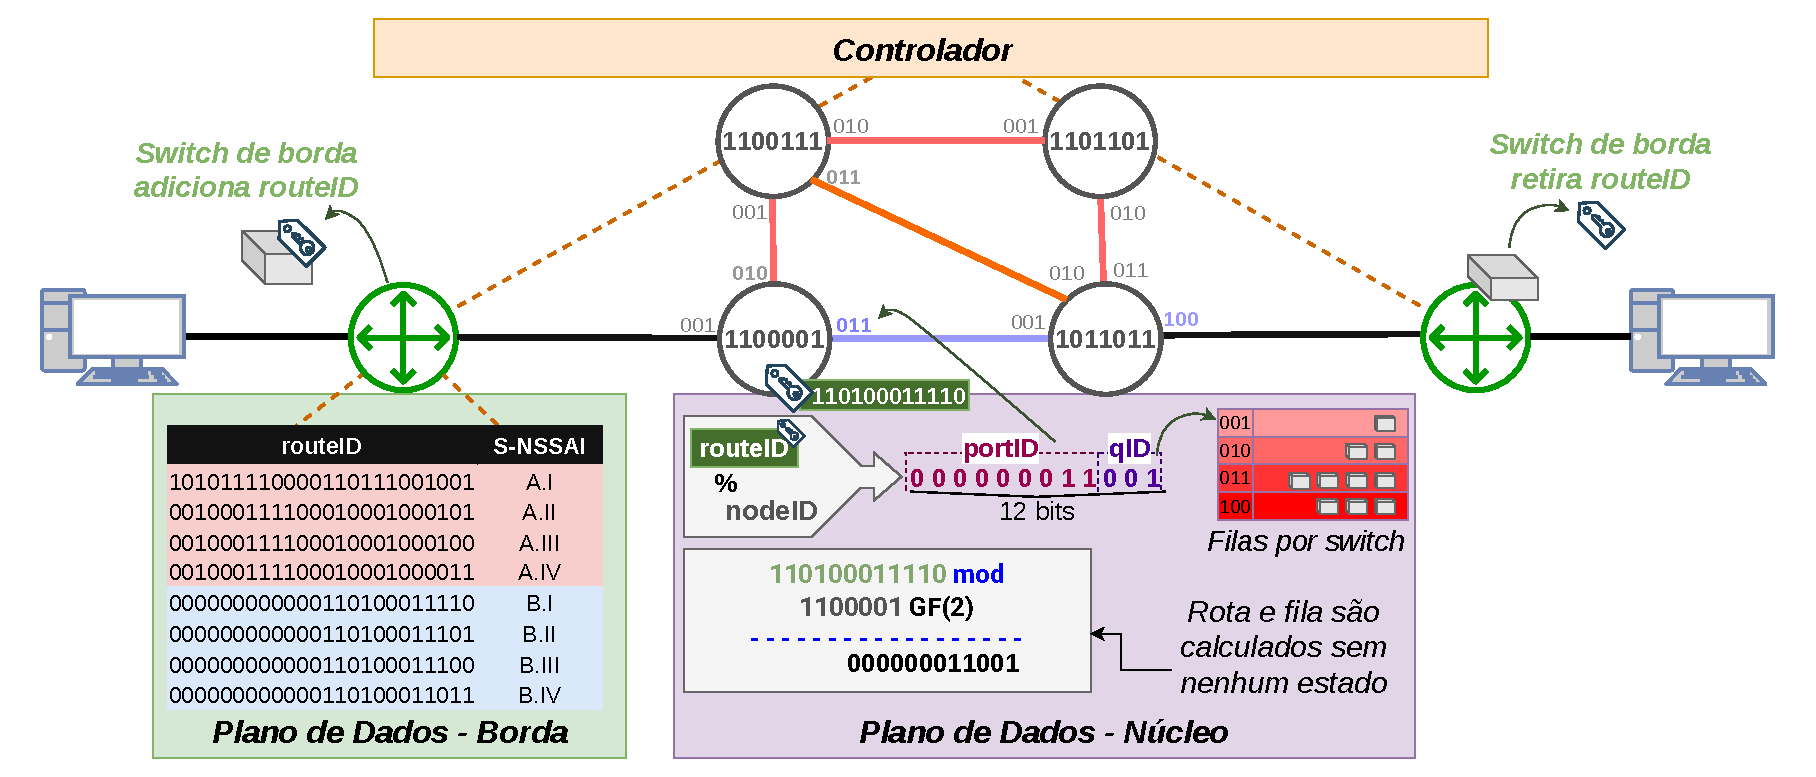
\includegraphics[width=\textwidth]{figuras/Arquitetura SPolKA.pdf}
    \captionsetup{justification=centering}
    \caption{Arquitetura \nome.}
    \label{fig:polka_example}
\end{figure}

A Figura~\ref{fig:polka_example} exemplifica o mecanismo descrito em uma topologia contendo dois nós de núcleo, cujos identificadores atribuídos pelo Controlador são os polinômios $s_1(t) = t^6 + t^5 + 1$ (representado em binário por $1100001$) e $s_2(t) = t^6 + t^4 + t^3 + t + 1$ ($1011011$). Para estabelecer o caminho $s_1 \rightarrow s_2$ com políticas específicas de enfileiramento em cada salto, o Controlador aplica o CRT polinomial e obtém o rótulo $R(t) = 110100011110$, associando-o ao identificador S-NSSAI na tabela de fluxo da borda de ingresso.

Quando o pacote alcança o primeiro nó de núcleo ($s_1$), o comutador executa a divisão polinomial em $GF(2)$ de $R(t) = 110100011110$ por $s_1(t) = 1100001$, extraindo o resto $o_1(t) = 000000011001$. Conforme ilustrado na decomposição do resultado de 12 bits, os 9 bits mais significativos ($000000011$) instruem o plano de dados a encaminhar o pacote pela porta física 3, ao passo que os 3 bits menos significativos ($001$) direcionam o pacote à fila de prioridade 1 daquela interface. O mesmo procedimento ocorre de forma independente no nó subsequente ($s_2$) utilizando seu próprio \nodeID, até que o switch de borda de egresso remova o cabeçalho do \routeID\ e entregue o pacote original.

\begin{quadro}[htb]
    \centering
    \caption{Função de cálculo do rótulo SPolKA em linguagem P4}
    \label{quad:codigo_controle}
    \begin{lstlisting}[language=P4]
        action srcRoute_nhop() {
            bit<16> nresult;
    
            // 1. Extração dos 160 bits mais significativos do routeId por deslocamento à direita
            bit<160> ndata = meta.routeId >> 16;
            
            // 2. Truncamento direto para obtenção dos 16 bits menos significativos (termo independente)
            bit<16> dif = (bit<16>)meta.routeId;
    
            // 3. Cálculo do resto da divisão polinomial em GF(2) via unidade de CRC-16 customizado,
            // utilizando constantes literais para otimizar a alocação de registradores
            hash(nresult,
                 HashAlgorithm.crc16_custom,
                 16w0,           // Valor base (offset) nulo
                 {ndata}, 
                 64w8589934592); // Limite superior do domínio de saída (2^33)
    
            // 4. Composição do polinômio de saída o_i(t) via adição modular (XOR)
            bit<16> nlabel = nresult ^ dif;
    
            // 5. Fatiamento de bits (bit-slicing) para decodificação simultânea de encaminhamento e QoS:
            meta.port = (bit<9>)nlabel[11:3]; // Bits [11:3] determinam o identificador da porta de saída (portID)
            meta.qid  = (bit<3>)nlabel[2:0];  // Bits [2:0] especificam o identificador da fila de serviço (qID)
        }
    \end{lstlisting}
    \fonte{Elaborado pelo autor (2026), adaptado de \textcite{nerds_polka}.}
\end{quadro}